\begin{figure}[htbp]
    \centering
    \definecolor{mercurygray}{RGB}{105,105,105}
    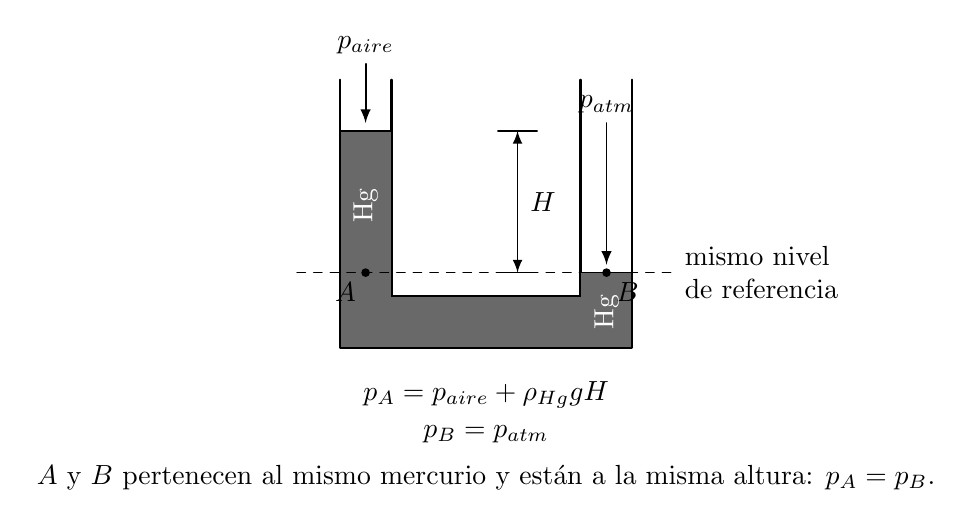
\begin{tikzpicture}[x=1cm,y=1cm,line cap=round,line join=round]
        % Manómetro en U conectado al aire del depósito por la izquierda
        \draw[line width=0.8pt]
            (1.00,3.65) -- (1.00,0.25) -- (4.70,0.25) -- (4.70,3.65);
        \draw[line width=0.8pt]
            (1.65,3.65) -- (1.65,0.90) -- (4.05,0.90) -- (4.05,3.65);

        % Mercurio: nivel izquierdo más alto que el derecho
        \fill[mercurygray] (1.01,0.26) rectangle (1.64,3.00);
        \fill[mercurygray] (1.64,0.26) rectangle (4.06,0.89);
        \fill[mercurygray] (4.06,0.26) rectangle (4.69,1.20);
        \draw[line width=0.5pt] (1.01,3.00) -- (1.64,3.00);
        \draw[line width=0.5pt] (4.06,1.20) -- (4.69,1.20);

        % Presiones sobre las superficies del mercurio
        \draw[line width=0.7pt,-latex] (1.32,3.85) -- (1.32,3.10);
        \node[above] at (1.32,3.85) {$p_{\text{aire}}$};
        \draw[line width=0.7pt,-latex] (4.38,3.10) -- (4.38,1.30);
        \node[above] at (4.38,3.10) {$p_{\text{atm}}$};

        % Diferencia de niveles H
        \draw[latex-latex,line width=0.6pt] (3.25,1.20) -- (3.25,3.00);
        \draw[line width=0.45pt] (3.00,1.20) -- (3.50,1.20);
        \draw[line width=0.45pt] (3.00,3.00) -- (3.50,3.00);
        \node[right] at (3.29,2.10) {$H$};

        % Puntos A y B al mismo nivel dentro del mercurio
        \draw[dashed,line width=0.55pt] (0.45,1.20) -- (5.25,1.20);
        \fill (1.32,1.20) circle (0.055);
        \fill (4.38,1.20) circle (0.055);
        \node[below left] at (1.32,1.20) {$A$};
        \node[below right] at (4.38,1.20) {$B$};
        \node[right,align=left] at (5.25,1.20) {mismo nivel\\de referencia};

        \node[rotate=90,text=white] at (1.32,2.05) {Hg};
        \node[rotate=90,text=white] at (4.38,0.70) {Hg};

        % Balance hidrostático desde cada superficie hasta la referencia
        \node[align=center] at (2.85,-0.35)
            {$p_A=p_{\text{aire}}+\rho_{\text{Hg}}gH$};
        \node[align=center] at (2.85,-0.85)
            {$p_B=p_{\text{atm}}$};
        \node[align=center] at (2.85,-1.40)
            {$A$ y $B$ pertenecen al mismo mercurio y están a la misma altura: $p_A=p_B$.};
    \end{tikzpicture}
    \caption{Balance de presión en un mismo nivel del mercurio.}
\end{figure}
